\chapter{全同粒子}
\section{两个粒子的相互作用体系}
前面我们一直讨论的系统都只有一个粒子, 如果现在又加入了一个粒子, 自由度变成了$6$, 体系的波函数应该用$\Psi(\mathbf{r}_1,\mathbf{r}_2,t)$去描述。我们首先可以断言体系的哈密顿算符可以写为:
\[\hat{H}=\frac{{\hat{p}_1}^2}{2m_1}+\frac{{\hat{p}_2}^2}{2m_2}+V(\mathbf{r}_1,\mathbf{r}_2,t)\]
故薛定谔方程写为:
\begin{equation}
    i\hbar\frac{\partial }{\partial t}\Psi(\mathbf{r}_1,\mathbf{r}_2,t)=\left[-\frac{\hbar^2}{2m_1}\nabla_1^2-\frac{\hbar^2}{2m_2}\nabla_2^2+V(\mathbf{r}_1,\mathbf{r}_2,t)\right]\Psi(\mathbf{r}_1,\mathbf{r}_2,t)
\end{equation}
其中$\nabla_1\equiv\frac{\partial}{\partial\mathbf{r}_1}$, 而且波函数的概率诠释也很显然, 它表示\textbf{在$\mathbf{r}_1$附近测量到粒子1\uwave{并且}在$\mathbf{r}_2$附近测量到粒子2}的概率为:
\begin{equation}
    \left|\Psi(\mathbf{r}_1,\mathbf{r}_2,t)\right|^2d^3r_1d^3r_2
\end{equation}

现在如果哈密顿算符不显含时间, 我们仍旧可以分离出时间项进行求解:
\[\Psi(\mathbf{r}_1,\mathbf{r}_2,t)=\sum\psi_n(\mathbf{r}_1,\mathbf{r}_2)e^{iE_nt/\hbar}\]
其中$\psi_n(\mathbf{r}_1,\mathbf{r}_2)$由下面的定态薛定谔方程给出:
\begin{equation}
    \label{eq:5.3}
    \left[-\frac{\hbar^2}{2m_1}\nabla_1^2-\frac{\hbar^2}{2m_2}\nabla_2^2+V(\mathbf{r}_1,\mathbf{r}_2)\right]\psi_n=E_n\psi_n
\end{equation}

上面的方程一般来说求解是及其困难的, 但是对于两种特殊情况, 两个粒子的问题实际上可以化简为一个粒子体系的问题。
\subsubsection*{两个粒子之间没有相互作用}
这也就是说, $V(\mathbf{r}_1,\mathbf{r}_2)$可以完全分离:
\[V(\mathbf{r}_1,\mathbf{r}_2)=V_1(\mathbf{r}_1)+V_2(\mathbf{r}_2)\]
这时, 波函数可以分离变量:
\[\psi(\mathbf{r}_1,\mathbf{r}_2)=\psi_1(\mathbf{r}_1)\psi_2(\mathbf{r}_2)\]
方程\ref{eq:5.3}可以写为:
\begin{align*}
    &-\frac{\hbar^2}{2m_1}\nabla_1^2\psi_1+V_1(\mathbf{r}_1)\psi_1=E_1\psi_1\\
    &-\frac{\hbar^2}{2m_2}\nabla_2^2\psi_2+V_2(\mathbf{r}_2)\psi_2=E_2\psi_2
\end{align*}
且$E_1+E_2=E$。显然, 现在双粒子体系问题变成了两个单粒子体系问题, 比如粒子1处于本征态$\psi_a$, 能量为$E_a$, 粒子2处于本征态$\psi_b$, 能量为$E_b$。则整个体系波函数就应该为:
\[\Psi\left(\mathbf{r}_{1}, \mathbf{r}_{2}, t\right)=\psi_{a}\left(\mathbf{r}_{1}\right) \psi_{b}\left(\mathbf{r}_{2}\right) e^{-i\left(E_{a}+E_{b}\right) t / \hbar}
=\Psi_1(\mathbf{r}_{1})\Psi_2(\mathbf{r}_{2})\]

是总能量$E=E_a+E_b$对应的本征矢。目前看来一切的推导都很合理, 但是别忘了, 薛定谔是线性方程, 所以本征态的叠加态也是体系可能处于的状态, 一旦涉及到多个单粒子体系的本征态, 事情就开始变得有些微妙了。
比如在合适的初始条件下, 粒子的波函数假设是:
\[\Psi\left(\mathbf{r}_{1}, \mathbf{r}_{2}, t\right)=\frac{3}{5} \Psi_{a}\left(\mathbf{r}_{1}, t\right) \Psi_{b}\left(\mathbf{r}_{2}, t\right)+\frac{4}{5} \Psi_{c}\left(\mathbf{r}_{1}, t\right) \Psi_{d}\left(\mathbf{r}_{2}, t\right)\]

这个波函数演化是满足薛定谔方程的, 那么如果在这个体系中去测量粒子1, 可能得到$E_a$(概率为$\frac{9}{25}$)或者$E_c$(概率为$\frac{16}{25}$), 单独测量$E_2$也是随机得到$E_b$或者$E_d$, 但是一旦
当我们测量到$E_1=E_a$, 体系将不可避免地坍缩到$\psi_a\psi_b$这个态, 这时我们可以断定测量$E_2$得到的一定是$E_b$, 失去了随机性。这种量子层面上神奇的粒子间的“互相纠缠”效应, 我们称体系
处于一个\textbf{纠缠态(entanglement)}。比如最初用来说明这个问题的典例, 就是双$1/2$粒子的单重态$\ket{0,0}$, 它无法写成单个粒子的态的直积形式, 比如
\[\frac{1}{\sqrt{2}}\left(\ket{\uparrow\uparrow}+\ket{\downarrow\downarrow}\right)=\frac{1}{\sqrt{2}}\left(\ket{\uparrow}+\ket{\downarrow}\right)\otimes\ket{\uparrow}\]
这个态就没有像$\ket{0,0}$一样纠缠, 而是如$\Psi_a\Psi_b$一般。

量子纠缠是一个非常复杂深奥的问题, 当时爱因斯坦先提出了这个问题来质疑量子力学的完备性, 这里不展开解释。

\subsubsection*{中心势场}
这时势能相退化为:
\[V(\mathbf{r}_1,\mathbf{r}_2)\rightarrow V(\left|\mathbf{r}_1-\mathbf{r}_2\right|)\]

参考我们经典力学中研究二体运动的思路, 首先我们改用质心坐标$\mathbf{R}$和相对坐标$\mathbf{r}$去描述系统, 我们这里也作坐标变换, 用这两个矢量去描述系统波函数。根据:
\[\mathbf{R}\equiv\frac{m_1\mathbf{r}_1+m_2\mathbf{r}_2}{m_1+m_2},\mathbf{r}=\mathbf{r}_1-\mathbf{r}_2,\mu\equiv\frac{m_1m_2}{m_1+m_2}\]
得到:
\[r_1=\mathbf{R}+\frac{\mu}{m_1}\mathbf{r},r_2=\mathbf{R}-\frac{\mu}{m_2}\mathbf{r}\]
且微分算符$\nabla$:
\[\nabla_1=\frac{\mu}{m_2}\nabla_R+\nabla_r,\nabla_2=\frac{\mu}{m_1}\nabla_R-\nabla_r\]
关于$\psi(\mathbf{R},\mathbf{r})$定态薛定谔方程变为:
\begin{equation}
    -\frac{^2}{2(m_1+m_2)}\nabla_R^2\psi-\frac{\hbar^2}{2\mu}\nabla_r^2\psi+V(\mathbf{r})\psi=E\psi
\end{equation}
然后现在对$\psi$分离变量求解方程, $\psi(\mathbf{R},\mathbf{r})=\psi_R(\mathbf{R})\psi_r(\mathbf{r})$:
\begin{align*}
    \left.\begin{array}{r}
        -\frac{\hbar^{2}}{2\left(m_{1}+m_{2}\right)} \nabla^{2} \psi_{R}=E_{R} \psi_{R} \\ 
       -\frac{\hbar^{2}}{2 \mu} \nabla^{2} \psi_{r}+V(\mathrm{r}) \psi_{r}=E_{r} \psi_{r}
      \end{array}\right\}E_R+E_r=E
\end{align*}

可见, “质心”位矢$R$的波函数正是自由粒子波函数, 和我们在经典力学里面预测的质心保持匀速直线运动相一致。相对位矢的波函数就是前面解氢原子的球谐函数加上径向解, 只要把电子质量$m_e$改为约化质量$\mu$即可。
\subsection{玻色子和费米子}
现在我们假设粒子1和粒子2分别处于$\psi_a$和$\psi_b$那么根据前面的讨论, 总的系统波函数应该为两者乘积\footnote{这里我们讨论定态, 忽略时间项}:
\begin{equation}
    \label{eq:5.5}
    \psi(\mathbf{r}_1,\mathbf{r}_2)=\psi_a(\mathbf{r}_1)\psi_b(\mathbf{r}_2)
\end{equation}  

打住, 我们现在一直在讨论粒子1和粒子2, 说它们分别处于两个态, 如果说一个是氢原子, 一个是氦原子, 那还好, 我们不会搞混, 我们可以完全区分这两个粒子。但是要是你面对的是两个电子呢?你还能区分吗?
在经典力学里面, 当然是可以的, 就算两个球做工完全一致, 外观看来完全没有差异, 但是在经典力学层面上我们始终可以追踪每个单独的球从而区分它们。但是基本粒子却是\textbf{全同的}, 意思就是无论如何你都不能区分它们, 这
和不确定性原理一样, 不是一个技术上的难题。在量子力学里面, 一旦我们进行了测量, 就不可避免的影响了整个系统。对于全同粒子我们不能再说某个粒子处于$\psi_a$, 另
一个处于$\psi_b$, 我们只能说两个粒子中有一个处于$\psi_a$, 有一个处于$\psi_b$, 而且两个粒子的地位完全等同, 我们无法区分。全同粒子假设目前已经经历了无数实验验证, 这里我们姑且就当作公理。

既然现在两个电子不能区分了, 那么\ref{eq:5.5}也就失去了意义, 我们现在应该去构造关于$\mathbf{r}_1$和$\mathbf{r}_2$交换对称的波函数, 注意这里包含反对称, 因为这样相当于只是差了个相位因子。
所以有下面的两种构造方式\footnote{注意这里实际上有很大的漏洞, 我们目前还没有讨论自旋部分, 其实\textbf{并不是}说费米子的波函数一定要反对称, 我们说的对称反对称是相较于粒子空间波函数和自旋整体而言的, 后面我们将会看到, 如果两个电子的自旋是反对称的, 那么它们也会处在对称的空间波函数状态。这里没有考虑自旋, 只是先初步有一个费米子玻色子的量子态对称性概念。}:
\begin{equation}
    \label{eq:5.6}
    \psi_\pm(\mathbf{r}_1,\mathbf{r}_2)=A\left[\psi_a(\mathbf{r}_1)\psi_b(\mathbf{r}_2)\pm\psi_b(\mathbf{r}_1)\psi_a(\mathbf{r}_2)\right]
\end{equation}

显然$\psi_+(\mathbf{r}_1,\mathbf{r}_2)=\psi_+(\mathbf{r}_2,\mathbf{r}_1)$, 满足这种对称性的粒子称为\textbf{玻色子(bosons)};另外, $\psi_-(\mathbf{r}_1,\mathbf{r}_2)=-\psi_-(\mathbf{r}_2,\mathbf{r}_1)$, 满足反对称的称为
\textbf{费米子(fermions)}。而且有下面的\uwave{经验规律}\footnote{要完整解释只能用量子场论}:
\begin{theorem}{自旋-统计定理}
    \begin{itemize}
        \item 自旋量子数$s$为整数的粒子是\textbf{玻色子}, 满足玻色-爱因斯坦统计
        \item 自旋量子数$s$为半整数的粒子是\textbf{费米子}, 满足费米-狄拉克统计
    \end{itemize}
\end{theorem}

现在如果两个粒子始终处于完全相同的状态, 也就是说\ref{eq:5.6}中有$\psi_a=\psi_b$。对于玻色子
\[\psi_+(\mathbf{r}_1,\mathbf{r}_2)=\psi_a(\mathbf{r}_1)\psi_b(\mathbf{r}_2)\]
但是对于费米子\footnote{我们这里的讨论少了粒子的自旋, 当然真实情况是包含自旋的}:
\[\psi_-(\mathbf{r}_1,\mathbf{r}_2)=0\]
这就是熟知的\textbf{泡利不相容原理}。
\begin{theorem}{泡利不相容原理}
    两个(或以上)全同的\textbf{费米子}不能处于相同的量子态
\end{theorem}
那根据泡利不相容原理, 难道两个氢原子里面的电子就不能都处于基态了吗?这显然是荒谬的, 就拿我们上面的例子来说, $\psi_-=0$的条件是$\psi_a=\psi_b$也就是
$\psi_a(\mathbf{r}_1)=\psi_b(\mathbf{r}_1)$且$\psi_a(\mathbf{r}_2)=\psi_b(\mathbf{r}_2)$, 对于两个相隔$\mathbf{r}$的氢原子, 它们的电子都处于基态, 相应的波函数分别是:
\[\psi_a(\mathbf{r}_1)=\psi_{100}(\mathbf{r}_1), \psi_b(\mathbf{r}_2)=\psi_{100}(\mathbf{r}_2-\mathbf{r})\]

显然这里不再有$\psi_a=\psi_b$, 虽然两个电子确实是都处于氢原子基态。但是对于同一个氦原子, 在高中化学中就接触到同一个轨道上的两个电子\footnote{这里说的都是基态, 也就是$n=1$, 那么$\ell=m=0$}, 必定一个自旋向上, 一个自旋向下。
\subsection{交换力}
我们继续考虑两个粒子, 现在只考虑一维情况。如果两个粒子是可以去区分的, 其中一个处于$\psi_a$另一个处于$\psi_b$而且这两个态是正交归一的。在没有纠缠的情况下, 总的态可以写成:
\[\psi(x_1,x_2)=\psi_a(x_1)\psi_b(x_2)\]
我们现在计算一下两个粒子之间的平均距离:
\[\Braket{\left(x_1-x_2\right)^2}=\Braket{x_1^2}+\Braket{x_2^2}-2\Braket{x_1}\Braket{x_2}\]
对于两个可区分的粒子显然有\footnote{注意这里我并没有用$\braket{x_1^2}_a$去指代$\int x_1^2|\psi_a(x_1)|^2dx_1$, 因为$x_1$只是一个类似于哑标的中间记号, 这样写有助于后面的化简。}:
\begin{align*}
    &\braket{x_1^2}=\int x_1^2|\psi_a(x_1)|^2dx_1\int |\psi_b(x_2)|^2dx_2=\braket{x^2}_a\\
    &\braket{x_1^2}=\int |\psi_a(x_1)|^2dx_1\int x_2^2 |\psi_b(x_2)|^2dx_2=\braket{x^2}_b\\
    &\braket{x_1x_2}=\int x_1x_2|\psi_a(x_1)|^2|\psi_b(x_2)|dx_1dx_2=\braket{x}_a\braket{x}_b
\end{align*}
故对于可分辨的两个粒子:
\begin{equation}
    \label{eq:5.7}
    \Braket{\left(x_1-x_2\right)^2}=\braket{x^2}_a+\braket{x^2}_b-\braket{x}_a\braket{x}_b
\end{equation}

但是如果是两个全同的玻色子或是费米子, 根据我们前面所说的这要求我们必须去构造堆成或是反对称的波函数, 也就是说:
\[\psi_\pm(x_1,x_2)=\frac{1}{\sqrt{2}}\left(\psi_a(x_1)\psi_b(x_2)\pm\psi_b(x_1)\psi_a(x_2)\right)\]
这个时候我们再去计算:
\begin{equation}
   \begin{aligned}
        \left\langle x_{1}^{2}\right\rangle=& \frac{1}{2}\left[\int x_{1}^{2}\left|\psi_{a}\left(x_{1}\right)\right|^{2} d x_{1} \int\left|\psi_{b}\left(x_{2}\right)\right|^{2} d x_{2}\right.\\
        &\left.+\int x_{1}^{2}\left|\psi_{b}\left(x_{1}\right)\right|^{2} d x_{1} \int\left|\psi_{a}\left(x_{2}\right)\right|^{2} d x_{2} \right.\\
        &\left.\pm \int x_{1}^{2} \psi_{a}\left(x_{1}\right)^{*} \psi_{b}\left(x_{1}\right) d x_{1} \int \psi_{b}\left(x_{2}\right)^{*} \psi_{a}\left(x_{2}\right) d x_{2}\right. \\
        &\left.\pm \int x_{1}^{2} \psi_{b}\left(x_{1}\right)^{*} \psi_{a}\left(x_{1}\right) d x_{1} \int \psi_{a}\left(x_{2}\right)^{*} \psi_{b}\left(x_{2}\right) d x_{2}\right] \\
        =& \frac{1}{2}\left[\left\langle x^{2}\right\rangle_{a}+\left\langle x^{2}\right\rangle_{b} \pm 0 \pm 0\right]=\frac{1}{2}\left(\left\langle x^{2}\right\rangle_{a}+\left\langle x^{2}\right\rangle_{b}\right)
    \end{aligned} 
\end{equation}
同理, 有:
\begin{equation}
    \braket{x_2^2}=\frac{1}{2}\left(\left\langle x^{2}\right\rangle_{b}+\left\langle x^{2}\right\rangle_{a}\right)
\end{equation}
最后计算交叉项:
\begin{equation}
    \begin{aligned}
        \left\langle x_{1} x_{2}\right\rangle=& \frac{1}{2}\left[\int x_{1}\left|\psi_{a}\left(x_{1}\right)\right|^{2} d x_{1} \int x_{2}\left|\psi_{b}\left(x_{2}\right)\right|^{2} d x_{2}\right.\\
        &\left.+\int x_{1}\left|\psi_{b}\left(x_{1}\right)\right|^{2} d x_{1} \int x_{2}\left|\psi_{a}\left(x_{2}\right)\right|^{2} d x_{2}\right. \\
        &\left. \pm \int x_{1} \psi_{a}\left(x_{1}\right)^{*} \psi_{b}\left(x_{1}\right) d x_{1} \int x_{2} \psi_{b}\left(x_{2}\right)^{*} \psi_{a}\left(x_{2}\right) d x_{2}\right. \\
        &\left.\pm \int x_{1} \psi_{b}\left(x_{1}\right)^{*} \psi_{a}\left(x_{1}\right) d x_{1} \int x_{2} \psi_{a}\left(x_{2}\right)^{*} \psi_{b}\left(x_{2}\right) d x_{2}\right] \\
        =& \frac{1}{2}\left(\langle x\rangle_{a}\langle x\rangle_{b}+\langle x\rangle_{b}\langle x\rangle_{a} \pm\langle x\rangle_{a b}\langle x\rangle_{b a} \pm\langle x\rangle_{b a}\langle x\rangle_{a b}\right) \\
        =&\langle x\rangle_{a}\langle x\rangle_{b} \pm\left|\langle x\rangle_{a b}\right|^{2}
    \end{aligned}
\end{equation}
其中:
\begin{equation}
    \label{eq:5.11}
    \langle x\rangle_{a b} \equiv \int x \psi_{a}(x)^{*} \psi_{b}(x) d x
\end{equation}
故对于全同粒子有:
\begin{equation}
    \Braket{\left(x_1-x_2\right)^2}=\Braket{x^2}_a+\Braket{x^2}_b-2\Braket{x}_a\Braket{x}_b\mp 2|\Braket{x}_{ab}|^2
\end{equation}

对照一下式\ref{eq:5.7}, 可以发现全同粒子多了一项$\mp 2|\Braket{x}_{ab}|^2$, 对于玻色子, 这一项倾向于让粒子相互靠近, 而对于费米子, 这一项倾向于让粒子相互远离。
就\uwave{好像}是它们之间有一股神奇的作用力一样, 我们称之为\textbf{交换力}。但是请特别注意, 交换力并不是真实存在的我们通常意义上的四大基本作用力之一或其某种表现, 而是纯粹的
由于费米子和玻色子的波函数对称性导致的几何结果, 而且是一种纯粹的量子效应。

有一种情况可以使得修正项\ref{eq:5.11}贡献为0, 那就是当两个波函数没有“重叠”的地方, 或者说通常意义下的两个粒子隔得很远。比如一个电子在武大一个电子在华科, 那么
这两个电子的波函数由于隔得很远基本上可以认为相乘之后总是0, 那么这个时候无论我们是直接使用波函数$\psi_a\psi_b$去描述, 还是使用对称化后的波函数$\psi_\pm$去描述都是一样的, 没有差别。
所以, 原则上虽然整个宇宙的电子都是全同的, 看起来我们不能只单单研究其中一个, 但是只要两个电子充分隔离, 我们在实际操作中就可以认为这两个电子是可以分辨的。所以我们可以明确的说\uwave{武大实验室的哪个电子}, 或者
\uwave{华科实验室的哪个电子}。但是在原子尺度范围内的两个电子, 我们就必须去考虑它们之间的全同粒子效应了。
\subsubsection*{共价键}
交换力的一个重要表现就是化学中的化学键, 我们考虑最简单的氢气分子$\mathrm{H}_2$。成键的是环绕两个质子的两个电子, 假设它们都处于基态。两个电子构成了一个全同粒子体系,
如果描述它们的波函数是完全对称的$\psi_+$, 那么根据上面关于交换力的论述, 电子会在两个氢原子核的连线中点处聚集, 聚集的负电荷就倾向于把两个质子向中间吸引, 这样就使得两个氢原子
牢牢地结合在了一起, 这便是化学键的本质(下图\ref{fig:5.1})。用化学上的话说就是电子云(波函数)的重叠, 这样$\braket{x}_{ab}\neq 0$。反之, 如果波函数是反对称的$\psi_-$, 负电荷就倾向于分散
这样分子便会被撕裂, 而不是聚合。
\begin{figure}[htbp]
    \centering
    \subfigure[对称结构产生吸引力] %第一张子图
    {
        \begin{minipage}{6cm}
        \centering          %子图居中
        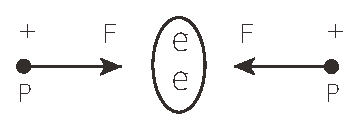
\includegraphics[scale=0.6]{fig/5-1-a.eps}  
        \end{minipage}
    }
    \subfigure[反对称结构产生排斥力] %第二张子图
    {
        \begin{minipage}{6cm}
        \centering      %子图居中
        \includegraphics[scale=0.6]{fig/5-1-b.eps}   
        \end{minipage}
    }
    \caption{化学键的本质}   %大图名称
    \label{fig:5.1}  %图片引用标记
\end{figure}

呃等等, 我们前面不是说了电子是费米子吗, 这样描述它们的波函数应该是$\psi_-$啊!所以化学家骗我们了, 分子间根本不能成键!这句话当然是错的, 因为我们还一直没考虑
粒子的自旋。我们现在加上粒子的自旋, 对于单个粒子, 总的量子态为:
\begin{equation}
    \psi(\mathbf{r})\chi
\end{equation}

注意我们这里直接写了个乘积, 这也是最简单的考虑, 表明粒子的自旋和粒子的空间坐标是完全分离的, 也就是说发现粒子自旋向上的概率不受粒子发现位置的影响。对于两个粒子
组成的系统, 我们把自旋加进来:
\begin{equation}
    \psi(\mathbf{r}_1,\mathbf{r}_2)\chi(1,2)
\end{equation}

其中$\chi(1,2)$是由我们$\S4\mbox{-}6$中就讨论过的两个自旋体系的自旋态, 态空间基底是张量积空间可以用耦合基底$\ket{s,m}$表示, 也可以用未耦合的基底$\ket{s_1,s_2,m_1,m_2}$
表示, 其中基底之间的变换关系由CG系数确定。那么电子的反对称性要求应该是对于包含自旋的量子态而言:
\begin{equation}
    \psi(\mathbf{r}_2,\mathbf{r}_1)\chi(2,1)=-\psi(\mathbf{r}_1,\mathbf{r}_2)\chi(1,2)
\end{equation}
电子对体系是双$1/2$自旋体系, 那么如果$\chi(1,2)$是自旋三重态, 那显然空间波函数只能是反对称$\psi_-$形式, 这样的话确实电子对无法成键。但是如果$\chi(1,2)$
是单态$\ket{0,0}$, 那么显然空间波函数要求是对称的$\psi_+$形式。这样电子对就可以成键了, 所以成键电子对的自旋都是“相反”的。而且从这里我们还可以进一步看出泡利不相容原理
并没有说两个电子的波函数必须不一样, 只要它们自旋一个是$\uparrow$一个是$\downarrow$就好。只是不能自旋和波函数都在同一状态。
\subsubsection*{对称化假设}
首先我们定义\textbf{置换算符}$\hat{P}$:
\begin{equation}
    \boxed{
        \hat{P}\ket{1,2}=\ket{2,1}
    }
\end{equation}

其中$\ket{1,2}$表示粒子1和粒子2构成的体系的量子态, 置换算符的作用就是交换两个粒子的角色, 或者说的更加实操一点, 就是把两个粒子所有的量的下标全部交换。
当然, 我们上面只是用双粒子体系来叙述, 类似的N个粒子组成的系统也可以类似定义。

对于全同粒子, 根据交换对称性, 描述它们的哈密顿算符一定是对称的, 也就是说$m_1=m_2$且$V(\mathbf{r}_1,\mathbb{r}_2,t)=V(\mathbf{r}_2,\mathbb{r}_1,t)$
我们得到:
\begin{equation}
    \label{eq:5.18}
    \left[\hat{P},\hat{H}\right]=0
\end{equation}
再根据\ref{广义欸费斯托定理}:
\begin{equation}
    \frac{d\Braket{\hat{P}}}{dt}=0
\end{equation}

也就是说如果粒子体系的量子态是对称的, 那么之后它们如何演化都还是对称的, 反对称亦然。对于两个可分辨粒子的体系, 它们的波函数也\textbf{可以}是对称的或者反对称的, 只要我们构造一个
体系, 使得描述这个体系的哈密顿量是对称的就行了, 那么\ref{eq:5.18}描述的对易关系仍旧成立, 仍然有波函数对称性与时间无关。注意, 我们对于可分辨的粒子体系, 我们是说它们
的量子态\textbf{可以}是对称形式的, 但是对于全同粒子, 他们的量子态\textbf{必须}是完全对称或者完全反对称的。下面我们要叙述的是一般的公理。
\begin{proposition}{对称化假设}
    在体系含有多个全同粒子时,只有其态空间中的某些右矢\footnote{我们用狄拉克符号叙述, 你也可以就说是量子态。}才能描述其物理状态, 根据全同粒子的性质, 这些物理右矢, 对于粒子的对换而言, 或是完全对称的, 或是完全反对称的. 我们称一类粒子为玻色子, 它们的物理右矢是对称的; 而称另一类粒子为费米子, 它们的物理右矢是反对称的.
    \begin{equation}
        \boxed{
            \ket{1,2,\ldots,i,\ldots,j,\ldots,n}=\pm\ket{1,2,\ldots,j,\ldots,i,\ldots,n}
        }
    \end{equation}
\end{proposition}
我们之前说的$\psi_\pm$的对称化构造是上述假设的特殊形式。

\section{原子}
我们现在来考虑一个一般的中性原子, 原子数为$Z$。注意, 由于核外电子质量远小于原子核的质量, 所以我们下面的讨论中可以认为原子核就是不动的, 电子受一个稳定的
有心势场作用。我们写下核外电子体系的哈密顿量:
\begin{equation}
    \hat{H}=\sum_{j=1}^{Z}\left\{-\frac{\hbar^{2}}{2 m} \nabla_{j}^{2}-\left(\frac{1}{4 \pi \epsilon_{0}}\right) \frac{Z e^{2}}{r_{j}}\right\}+\frac{1}{2}\left(\frac{1}{4 \pi \epsilon_{0}}\right) \sum_{i \neq k}^{Z} \frac{e^{2}}{\left|\mathbf{r}_{j}-\mathbf{r}_{k}\right|}
\end{equation}

上式中的第一项是电子的动能以及电子与原子核间相互作用的库伦势能, 第二项是核外电子之间的库伦排斥力导致的静电互能, 这些在经典电磁学中都已经详细讨论过了。
顺便说一句, 上面的式子显然是对于每两个指标交换对称的, 这符合我们前面的全同粒子假设。

哈密顿算符不显含时间, 所以我们可以空间时间变量分离, 去寻找定态方程的解:
\[\hat{H}\psi=E\psi\]

$Z=1$即氢原子的情况, 我们在上一章中已经详细讨论精确求解。但很遗憾, 对于$Z>1$的情形我们无法精确求解上面的方程, 烦人的就是最后一项电子之间的相互作用。我们只能
借助一些近似方法数值求解, 我们接下来就定性分析一下解的特征。

\subsection*{氦原子}
氦原子是$Z>1$里面最简单的情形:
\begin{equation}
    \hat{H}=\left\{-\frac{\hbar^{2}}{2 m} \nabla_{1}^{2}-\frac{1}{4 \pi \epsilon_{0}} \frac{2 e^{2}}{r_{1}}\right\}+\left\{-\frac{\hbar^{2}}{2 m} \nabla_{2}^{2}-\frac{1}{4 \pi \epsilon_{0}} \frac{2 e^{2}}{r_{2}}\right\}+\frac{1}{4 \pi \epsilon_{0}} \frac{e^{2}}{\left|\mathbf{r}_{1}-\mathbf{r}_{2}\right|}
\end{equation}
如果现在我们忽略最后一项电子之间的相互作用, 现在哈密顿量就简化为了两个粒子间无相互作用的情形。根据我们之前的说法, 这种情况是可以分离变量求解的, 可以完全化简为两个单独的单粒子体系问题, 
对每个单粒子体系求解后波函数相乘便得到了系统的解, 若是全同粒子体系, 进一步用前面的解构造出对称和反对称的解即可。

不难看出, 剩下要做的事情在上一章我们求解氢原子的时候就已经做完了, 现在我们只用照搬上一章的结果, 只是需要把$e^2$改成$Ze^2$即可。
\[\psi=\psi_{n\ell m}\psi_{n^\prime\ell^\prime m^\prime}\]

等等, 我们好像又没有考虑自旋。我们在求解空间波函数的时候确实不用考虑自旋, 因为哈密顿算符并没有对自旋有作用, 但是最后我们的结果应该包含自旋$\chi_(1,2)$。\footnote{我们目前都是最简单的考虑, 一是认为自旋和空间波函数之间没有耦合, 而且在三个或更多粒子的全同粒子体系中, 没有反对称的自旋态, 量子态的构造更加复杂, 是一系列线性组合。这里我们就考虑了最简单的氦原子, 总的量子态就直接是$\psi(\mathbf{r}_1,\mathbf{r}_2)\chi(1,2)$}
如果两个电子都处于基态, 那么\footnote{按照$e^2\rightarrow Ze^2$的变换, 显然玻尔半径变成原来的一半, 单个电子基态能量变成原来的四倍。}:
\[\psi_{0}\left(\mathbf{r}_{1}, \mathbf{r}_{2}\right)=\psi_{100}\left(\mathbf{r}_{1}\right) \psi_{100}\left(\mathbf{r}_{2}\right)=\frac{8}{\pi a^{3}} e^{-2\left(r_{1}+r_{2}\right) / a}\]

这是已经一个对称的空间波函数, 所以两个电子的自旋态应该是反对称的单态$\ket{0,0}$, 用化学家的话说就是两个电子自旋“相反”, 这也是泡利不相容原理所希望的。

体系基态能量为:
\[E_0=4(E_{0,\mathrm{H}}+E_{0,\mathrm{H}})=8\times(\SI{-13.6}{\eV})\approx\SI{-109}{\eV}\]

实验测得上面的值为$\SI{-78.975}{\eV}$, 相差还是蛮大的, 这也不难理解, 因为我们的近似做的实在是太粗略了。我们首先利用上面没有考虑电子对之间的相互作用粗略得出来的系统空间波函数
计算:
\begin{equation}
    \braket{\frac{1}{\left|\mathbf{r}_1-\mathbf{r}_2\right|}}=\int\frac{1}{|\mathbf{r}_1-\mathbf{r}_2|}|\psi_0(\mathbf{r}_1,\mathbf{r}_2)|^2d^3r_1d^3r_2
\end{equation}

上面这个积分比较难算, 但是我们可以充分利用波函数的球对称性, 我们先对$\mathbf{r}_2$积分, 重点来了, 这里根据波函数球对称性, 我们可以设积分时$\mathbf{r}_1$沿着极轴方向。尝试计算\footnote{如果你用不惯这个技巧, 直接直角坐标系或者换元计算也可以, 常规方法更不易出错。}:
\begin{equation}
    \int d^3r_1 \int \left(\sqrt{r_{1}^{2}+r_{2}^{2}-2 r_{1} r_{2} \cos \theta_{2}}\right)^{-1}\left[\frac{8}{\pi a^{3}} e^{-2\left(r_{1}+r_{2}\right) / a}\right]^2d^3r_2
\end{equation}
根据球坐标换元我们马上可以得到上面积分的结果为:
\begin{align*}
    \mathrm{Ans}&=\frac{512}{\pi a^6}\int d^3r_1\int_0^{+\infty}\frac{r_2^2 e^{\frac{4(r_1+r_2)}{a}}}{|r_1+r_2|+|r_1-r_2|}dr_2\\
    &=\int_0^{+\infty}\frac{32}{a^4}e^{-\frac{8r_1}{a}}frac{a(e^{\frac{4r_1}{a}}-1)-2r_1}{r_1}\cdot 4\pi r_1^2dr_1\\
    &=\boxed{\frac{5}{4a}}
\end{align*}
根据上面的算式我们可以估算基态能量的修正值为:
\begin{align*}
    \Delta E_0&\approx\frac{e^2}{4\pi\varepsilon_0}\braket{\frac{1}{\left|\mathbf{r}_1-\mathbf{r}_2\right|}}\\&=\frac{e^2}{4\pi\varepsilon_0}\left(\frac{5}{4a}\right)^{-1}\\
    &\approx\SI{34}{\eV}
\end{align*}
和前面计算出来的$\SI{-109}{\eV}$相加后得到$\SI{-75}{\eV}$, 这和测量值已经吻合的很好了。

我们再来简单的考虑一下激发态:\footnote{激发态必然是一个电子处于基态, 另一个电子处于激发态, 如果两个电子都处于激发态, 那么其中一个电子会向基态跃迁并发射能量, 使得另一个电子吸收能量电离!这样我们考虑的就不是$\mathrm{He}$原子了, 而是$\mathrm{He}^+$}
\[\psi=\psi_{100}\psi_{n\ell m}\]

我们根据这个可以构造对称和反对称波函数, 对于对称的波函数, 电子的自旋态是反对称的单重态, 我们把处于这个状态的氦原子称为\textbf{仲氦(parahelium)}。对于反对称的波函数, 自旋态处于
对称的三重态, 这个时候我们称之为\textbf{正氦(orthohelium)}。显然, 仲氦的能量要普遍高于正氦, 因为对称的波函数导致的结果是电子靠的更近, 所以对应的电子对之间的库伦势能也要更大, 所以整体
来看能量更大。

\subsubsection*{一点点化学}
高中阶段的化学和量子力学联系的最为紧密的就是原子的基态电子排布式了, 下面我们用量子力学的观点, 再来解释一下高中所学的那些化学家的语言。

首先这部分来说在原子物理的课程中也有所介绍, 但是一般来说都是给还未学过量子力学的人介绍, 所以相关的术语就还停留在玻尔的老的量子论阶段, 比如“电子轨道”这些。
我们知道对于多电子的情形我们是很难定量分析的, 所以接下来的分析都是定性的分析, 首先我们还是假设先不考虑电子之间的相互作用。这样我们可以继续利用氢原子的
波函数的解去描述电子, 如此看来, 每个电子的状态就可以利用三个量子数$n,\ell,m$去描述其轨道性质, 最后再加上其自旋性质, 使用其自旋磁量子数即可完全描述。

化学家喜欢把同一个能级(主量子数$n$相同)上的电子称作是同一个\textbf{壳层(Shell)}, 依次使用K,L,M,N,标记。根据泡利不相容原理, 不能同时有两个电子处在相同的电子态, 
那么根据第$n$能级的简并度$d(n)=n^2$, 再加上每组相同的量子数取值又有$\uparrow\&\downarrow$两种自旋状态\footnote{我们的讨论都是非常简化了的, 实际情况可以是这些态的线性组合, 但是不要紧, 总的线性无关态数目与我们讨论的没有差别。}。
故每个壳层最多可以容纳$2n^2$个电子, 那么元素周期表的每行元素数量为何是$2,8,8,18,\ldots$而不是$2,8,18,32,\ldots$呢?

电子的排布总是倾向于让整个原子的能量最低, 这样才最稳定, 经过上面的讨论, 确定每个电子能量的就是其主量子数, 在电子之间没有相互作用的时候也确实如此。这样来看只要
按照壳层顺序依次来排布注意自旋取向就行了。但是实际上电子之间的作用还是蛮大的, 就算是氦原子都有大约足足$\SI{34}{\eV}$的贡献, 而这一部分的能量主要就是由角量子数$\ell$
确定的。用化学家的术语, 每个壳层的电子有$n-1$种轨道, 由$\ell$的取值标记。$\ell=0$, s(sharp);$\ell=1$,p(pincipal);$\ell=2$,d(diffuse);$\ell=3$。
进一步, 这些轨道有不同的取向, 由磁量子数$m$取值确定。比如$s$轨道只有一种取值, $p$轨道由于$m$取值为$0,\pm 1$, 就有$p_x,p_y,p_z$三种取向。

可以说角量子数取值对应的是轨道角动量的大小, 且越大角动量越大, 而轨道角动量定性的看是趋向于把电子向外甩, 而电子越往外面甩\footnote{我们只是说了一种倾向, 并没有说就真的甩出去了, 所以电子还是在一个固定的壳层}, 其内层电子对原子核的
“屏蔽”作用越大\footnote{可以用原子实的观点去思考}, 导致外层电子“感觉”到的吸引力越小, 进而导致整体能量更大, 所以电子在某一壳层会尽量占据$\ell$较小的轨道, 直到上一个轨道被填满。
氩原子之后的钾原子和钙原子不填充满第三层, 从第四层开始填正是因为$n=3,\ell=3$的取值方式$\ell$已经足够大导致这样做由于电子之间的能量比较高, 还不如填到下一能层的$s$轨道总能量低。
然后从钪到锌又继续填充到第三层$d$轨道。

所以很多时候排布式只能依靠经验规则写出来, 再经过实验验证, 确实因为电子之间的相互作用给我们求解带来了不少麻烦。至于排布式具体怎么写, 这个化学课上已经讲过, 然后我们再
根据上面的量子力学背景分析就好了。
\section{固体}
中学就学过, 金属能导电是因为其中有些电子脱离了原子的束缚成为\textbf{自由电子}, 这些电子因为电场的作用在固体结构种移动便形成了电流。我们下面就是要用两种不同的模型基于量子力学的
原理去研究固体中电子的运动。它们只是固体理论中最最基础的理论。

\subsection{自由电子气理论}
这个模型中, 我们认为所有的电子都是在固体中自由运动的, 也就是说忽略电子之间的库伦斥力以及原子对电子的吸引力, 除了电子不能飞出固体边界这个条件。如果固体是一个
长方体\footnote{我们这里只是使用长方体模型去计算, 实际上我么后面推导出的\ref{eq:5.27},\ref{eq:5.28},\ref{eq:5.30},\ref{eq:5.32}对任何形状的固体都是适用的。}, 那么问题就是我们在$\S$4-1中就研究过的三维无限深势阱模型, 只是那里是正方体, 我们这里是更一般的长方体, 但也是分离变量法很快的就能求解出来:
\begin{equation}
    \psi_{n_{x} n_{y} n_{z}}=\sqrt{\frac{8}{l_{x} l_{y} l_{z}}} \sin \left(\frac{n_{x} \pi}{l_{x}} x\right) \sin \left(\frac{n_{y} \pi}{l_{y}} y\right) \sin \left(\frac{n_{z} \pi}{l_{z}} z\right)
\end{equation}
对应的定态能量\footnote{$\mathbf{k}$是波矢。}:
\begin{equation}
    \label{eq:5.25}
    E_{n_{x} n_{y} n_{z}}=\frac{\hbar^{2} \pi^{2}}{2 m}\left(\frac{n_{x}^{2}}{l_{x}^{2}}+\frac{n_{y}^{2}}{l_{y}^{2}}+\frac{n_{z}^{2}}{l_{z}^{2}}\right)=\frac{\hbar^{2} k^{2}}{2 m}
\end{equation}

\begin{figure}[htbp]
    \centering
    \includegraphics[scale=0.72]{fig/5-2.jpg}
    \caption{k-space}
    \label{fig:5-2}
\end{figure}

其中量子数的取值都是$1,2,3,\ldots$。为了形象的表示出电子可能所处的定态, 我们可以使用下面所谓“k-空间”的概念, 也便于我们后面进一步的计算。


如图\ref{fig:5-2}, 我们给定了$k_x,k_y,k_z$就相当于给定了电子的状态, 表现在图上就是一个交点, 所有的交点填满了整个直角坐标的第一卦限, 标记了电子的所有定态波函数
的可能情况。但是这是离散化的, 还是不方便我们后面的计算, 我们下面将它连续化。还记得化学里面数晶体的原子数密度吗?这里我们画了一个阴影部分, 在这一部分有八个顶点, 也就是八个定态, 
但是每个定态又被八个这样的体积所“共有”。所以总的来说这样一个体积内可以看作是平均有一个定态。我们如果把电子的自旋考虑进来, 那么图中的每个交点应该代表两个不同的量子态,
自旋向上自旋向下各一个, 平均一个态占据的“体积”也便是图中阴影部分的一半了。

根据泡利不相容原理, 自由电子在固体中只可能有两个电子处于相同的定态, 但具有相反的自旋态。我们现在考虑一个具有$N$个原子的体系, $N$具有阿伏伽德罗常数的
数量级, 平均每个原子贡献$d$个自由电子。所有的电子处于的量子态合起来看就是k-空间中占据的某个体积, 总能量应该趋于最小, 这应该是k-空间中的$1/8$球体。如下图\ref{fig:5-3}
所示。
\begin{figure}
    \centering
    \includegraphics{fig/5-3.jpg}
    \caption{固体中所有电子占据的态}
    \label{fig:5-3}
\end{figure}

注意, 严格来说这不是一个球体, 而是表面面有很多“锯齿”的球体, 但是因为电子数目很多, 所以越往外越接近球形, 我们下面的计算就按照球形来算也是很好的近似。
我们现在设这个${\raise0.5ex\hbox{$\scriptstyle 1$}\kern-0.1em/\kern-0.15em\lower0.25ex\hbox{$\scriptstyle 8$}}$球体的半径为$k_F$, 称为\textbf{费米半径}, 现在我们一方面可以利用费米半径
表示出它的体积, 然而这个体积和总的自由电子数目又是完全相关的, 我们前面把这些点阵“连续化”为点所占据的小盒子的方法就派上用场了:
\begin{equation}
    \frac{1}{8}\left(\frac{4}{3}\pi k_F^3\right)=\frac{1}{2}\left[Nd\left(\frac{\pi}{l_x}\right)\left(\frac{\pi}{l_y}\right)\left(\frac{\pi}{l_z}\right)\right]
\end{equation}
注意上面公式中出现的二分之一, 这是因为电子的两种不同自旋状态。\footnote{我们目前使用了很多不太严谨的说法, 比如电子的上下自旋这种说法, 只要牢记我们提的是自旋磁量子数的两种取值就行了, 当然实际上电子自旋可以处于两种状态的叠加态。}
定义$V\equiv l_xl_yl_z$即固体的体积, 得:
\begin{equation}
    \label{eq:5.27}
    k_{F}=\left(3 \rho \pi^{2}\right)^{1 / 3}
\end{equation}
其中$\rho\equiv\frac{Nd}{V}$可以认为是自由电子的数密度。

这个球体的表面对应的能量称为\textbf{费米能}, 是固体中的自由电子可能的最大能级。根据\ref{eq:5.25}
\begin{equation}
    \label{eq:5.28}
    E_{F}=\frac{\hbar^{2}}{2 m}\left(3 \rho \pi^{2}\right)^{2 / 3}
\end{equation}

我们还可以进一步计算自由电子的总能量$E_{tot}$, 我们考虑厚度为$dk$的球壳, 这部分体积内的量子态对应的能量为$\frac{\hbar^2k^2}{2m}$, 数目根据我们前面的体积算法为:
\begin{equation}
    2\frac{\frac{1}{8}\cdot4\pi k^2\cdot dk}{\pi^3/V}
\end{equation}
前面的2又是考虑了两种自旋取向。求和变成了积分:\footnote{你仔细一想就会明白, 我们这里本来是要对$N_A$数量级的电子求和, 和求积分的结果肯定是有出入的, 但好在我们这样一路的近似最终看起来也没多大偏差。}
\begin{equation}
    \label{eq:5.30}
    E_{\text {tot }}=\frac{\hbar^{2} V}{2 \pi^{2} m} \int_{0}^{k_{F}} k^{4} d k=\frac{\hbar^{2} k_{F}^{5} V}{10 \pi^{2} m}=\frac{\hbar^{2}\left(3 \pi^{2} N d\right)^{5 / 3}}{10 \pi^{2} m} V^{-2 / 3}
\end{equation}

这个能量和热学里面的气体的内能差不多意思, 我们就叫他电子气的内能吧。这个能量显然是和固体的体积相关的, “电子气”也会对\uwave{器壁}, 也就是固体表面产生压力, 我们假设这个压强是$P$。
我们用虚功原理来看待这个问题, 如果器壁现在因为电子气的压力产生微小形变$dV$。显然电子气对其做功大小为:$dW=-PdV$。而这应该正好等于电子气能量的变化:
\begin{equation}
    d E_{\mathrm{tot}}=-\frac{2}{3} \frac{\hbar^{2}\left(3 \pi^{2} N d\right)^{5 / 3}}{10 \pi^{2} m} V^{-5 / 3} d V=-\frac{2}{3} E_{\mathrm{tot}} \frac{d V}{V}
\end{equation}

所以可以计算出压强的大小:
\begin{equation}
    \label{eq:5.32}
    P=\frac{2}{3} \frac{E_{\text {tot }}}{V}=\frac{2}{3} \frac{\hbar^{2} k_{F}^{5}}{10 \pi^{2} m}=\frac{\left(3 \pi^{2}\right)^{2 / 3} \hbar^{2}}{5 m} \rho^{5 / 3}
\end{equation}

这个固有压强是支撑起固体使其不会塌缩的部分原因, 我们称之为\textbf{简并压(degeneracy pressure)}。这和电子之间的库仑斥力或是电子的热运动无关, 是一个
纯粹的量子力学结果, 是费米子的量子态的反对称性要求导致的, 也是泡利不相容原理的必然结果。天文学上的中子星的产生就跟引力塌缩突破简并压有关。

\subsection{价带结构}
如果按照我们前面的最简单的自由电子气模型, 那么所有的固体都应该是导体, 因为都或多或少有自由电子存在。所以我们现在要前进一点点, 把周期性的\footnote{这个周期性也很好理解, 因为晶体结构具有周期性}原子对电子的作用考虑进来。
但是我们依旧认为电子之间是没有相互作用的, 我们下面先考虑一维情形单个电子在周期性势场中的问题求解, 因为不考虑电子之间相互作用, 所以多个电子只需要把单个电子问题的解相乘即可。
\begin{define}{狄拉克梳}
    没啥好讨论的, 不过就是前面的狄拉克$\delta$函数加了个周期性而已
    \begin{equation}
        V(x)=\alpha \sum_{j=0}^{N-1} \delta(x-j a)
    \end{equation}
\end{define}
\begin{figure}
    \centering
    \begin{tikzpicture}[scale=0.4] %缩放,还可以设置xscale, yscale
        \draw[->](9,-0.7)--(9,6) node[above]{$V(x)$};
        \draw[->](0.8,0)--(29.2,0) node[below]{$x$};  % 画坐标轴
        \draw (9,0) node[below right]{$O$};
        \draw (3,0) node[below]{$-2a$};
        \draw[->,red] (3,0)--(3,4);
        \draw (6,0) node[below]{$-a$};
        \draw[->,red] (6,0)--(6,4);
        \draw[->,red] (9,0)--(9,4);
        \draw (12,0) node[below]{$a$};
        \draw[->,red] (12,0)--(12,4);
        \draw (15,0) node[below]{$2a$};
        \draw[->,red] (15,0)--(15,4);
        \draw (18,0) node[below]{$3a$};
        \draw[->,red] (18,0)--(18,4);
        \draw (21,0) node[below]{$4a$};
        \draw[->,red] (21,0)--(21,4);
        \draw (24,0) node[below]{$5a$};
        \draw[->,red] (24,0)--(24,4);
        \draw (27,0) node[below]{$6a$};
        \draw[->,red] (27,0)--(27,4);
    \end{tikzpicture}  
    \caption{狄拉克梳状函数}
    \label{fig:5.4}
\end{figure}
这个狄拉克梳状函数就是我们要面对的势场, 或许我们需要取$\alpha<0$才能描述原子核对电子的吸引性质, 不过我们现在仅仅只是想定性的去分析势场的周期性质到底会给我们带来什么, 所以
势场的具体性状我们并不是那么关心, 更关心它的周期性, 所以我们为了最大的简化我们的计算, 就选取$\alpha>0$的狄拉克梳状函数。

为了求解具有空间周期性的势场下的薛定谔方程, 我们首先介绍布洛赫(Bloch)定理\footnote{我们现在探讨的问题是空间周期性对解的影响, 在经典力学中曾经处理过
参数共振的问题, 那个时候是势场的时间周期性对解的影响, 那个时候也有和Bloch定理对应的Floquet理论, 整个问题的求解和这里也极为相似。}。
\begin{theorem}{Bloch's theorem}
    如果势场$V(x)$以$a$为周期, 那么定态薛定谔方程的解一定满足下面的性质:
    \begin{equation}
        \label{eq:5.34}
        \boxed{
            \psi(x+a)=e^{iqa}\psi(x)
        }
    \end{equation}
    其中$q$是与$x$无关(但与$E$有关)的一个常数。
\end{theorem}

可惜没有固体是无限大的, 所以严格意义上来说根本没有周期性的势场。所以这样的边界效应需要我们对Bloch定理进行修正, 不过好在固体的原子数目众多, 达到了$N_A$量级, 所以
这样的修正还算简单。我们现在考虑把x轴首位相连形成一个圆, 这个修正就是在这样的基础上有边界条件:
\begin{equation}
    \psi(x+Na)=\psi(x)
\end{equation}
$N$是原子数目。所以我们可以得到q必须满足:
\begin{equation}
    \label{eq:5.36}
    e^{iqNa}=1\Rightarrow q=\frac{n\pi}{Na},(n=0,\pm 1,\pm 2,\ldots)
\end{equation}

我们只需要解出$[0,a]$内的解, 其它区间内的解可以直接由\ref{eq:5.34}迭代得到。在$(0,a)$内有:
\begin{equation}
    \frac{d^2\psi}{dx^2}=-k^2\psi,k\equiv\frac{\sqrt{2mE}}{\hbar}
\end{equation}
驻波形式解为:
\begin{equation}
    \label{eq:5.38}
    \psi(x)=A\sin(kx)+B\cos(kx),x\in(0,a)
\end{equation}
再利用\ref{eq:5.34}我们得到$[-a,0]$内的解:
\begin{equation}
    \label{eq:5.39}
   \psi(x)=e^{-iqa}\left[A\sin k(x+a)+B\cos k(x+a)\right] ,x\in(-a,0)
\end{equation}
再根据波函数在$x=0$处的连续性:
\begin{equation}
    \label{eq:5.40}
    \psi(0^+)=\psi(0^-)\Rightarrow B=e^{-iqa}\left[A\sin ka+B\cos ka\right]
\end{equation}
然后再根据薛定谔方程在$0^-\sim 0^+$上积分得出$\delta$函数导致的一阶导在$0$附近的突变值:\footnote{在$\S$2-5中已经处理过很多次}
\begin{equation}
    \label{eq:5.41}
    \psi^\prime(0^+)-\psi^\prime(0^-)=\frac{2m\alpha}{\hbar^2}\psi(0)=\frac{2m\alpha}{\hbar^2}B
\end{equation}
对\ref{eq:5.38}和\ref{eq:5.39}求导后代入\ref{eq:5.41}得:
\begin{equation}
    \label{eq:5.42}
    kA-e^{-iqa}k\left(A \cos ka-B\sin ka\right)=\frac{2m\alpha}(\hbar^2) B
\end{equation}
将\ref{eq:5.40}和\ref{eq:5.42}联立求解得到:
\begin{equation}
    \label{eq:5.43}
    \cos qa=\cos z+\beta\frac{\sin z}{z}
\end{equation}
其中:
\[z\equiv ka, \beta\equiv\frac{m\alpha a}{\hbar^2} \]
方程\ref{eq:5.43}给出了$k$的可能取值, 也即能量取值。我们作下面函数的图像来分析:
\[f(z)=\cos z+\beta\frac{\sin z}{z}\]
\begin{figure}[htbp]
    \centering
    \begin{tikzpicture}[scale=0.7] %缩放,还可以设置xscale, yscale
        \draw (0,0) rectangle (5*pi,5.2*1.82);
        \draw[elegant,orange,domain=2.29524:5*pi] plot(\x,{1.82*cos(\x r) + 18.2*sin(\x r)/\x +2.6*1.82});
        \draw (0,0) node[below]{$0$};
        \draw (pi,0) node[below]{$\pi$};
        \draw (2*pi,0) node[below]{$2\pi$};
        \draw (3*pi,0) node[below]{$3\pi$};
        \draw (4*pi,0) node[below]{$4\pi$};
        \draw (5*pi,0) node[below]{$5\pi$};
        \draw (0,2.6*1.82) node[left]{$O$};
        \draw (0,2.6*1.82)--(5*pi,2.6*1.82) node[right]{$z$};
        \draw[help lines] (0,1.6*1.82)--(5*pi,1.6*1.82);
        \draw (0,1.6*1.82) node[left]{$-1$};
        \draw[help lines] (0,3.6*1.82)--(5*pi,3.6*1.82);
        \draw (0,3.6*1.82) node[left]{$1$};
        \draw[help lines] (pi,0)--(pi,5.2*1.82);
        \draw[help lines] (2*pi,0)--(2*pi,5.2*1.82);
        \draw[help lines] (3*pi,0)--(3*pi,5.2*1.82);
        \draw[help lines] (4*pi,0)--(4*pi,5.2*1.82);
        \filldraw[draw=blue!80,fill=blue!20,fill opacity=0.5] (2.62768,1.6*1.82) rectangle (pi,3.6*1.82);
        \filldraw[draw=blue!80,fill=blue!20,fill opacity=0.5] (5.30732 ,1.6*1.82) rectangle (2*pi,3.6*1.82);
        \filldraw[draw=blue!80,fill=blue!20,fill opacity=0.5] (8.06714 ,1.6*1.82) rectangle (3*pi,3.6*1.82);
        \filldraw[draw=blue!80,fill=blue!20,fill opacity=0.5] (10.9087 ,1.6*1.82) rectangle (4*pi,3.6*1.82);
        \filldraw[draw=blue!80,fill=blue!20,fill opacity=0.5] (13.8192 ,1.6*1.82) rectangle (5*pi,3.6*1.82);
    \end{tikzpicture}  
    \caption{$\beta=10$时$f(z)$的图像}
    \label{fig:5.5}
\end{figure}
\begin{figure}
    \centering
    \begin{tikzpicture}[scale=0.92]
        \draw[->] (0,0)--(14,0) node[below]{$E$};
        \draw (0,0) -- (0,3);
        \draw (0,3) -- (13.8,3);
        \fill[pattern=vertical lines,pattern color=blue]
        (0,0) rectangle (3.2,3);
        \fill[pattern=vertical lines,pattern color=blue]
        (6.1,0) rectangle (9.3,3);
        \fill[pattern=vertical lines,pattern color=blue]
        (10.6,0) rectangle (13.8,3);
        \draw[decorate,decoration={brace,mirror,amplitude=0.2cm},red] (0,0) -- (3.2,0)node[black,midway,yshift=-0.4cm]{允带};
        \draw[decorate,decoration={brace,mirror,amplitude=0.2cm},orange] (3.2,0) -- (6.1,0)node[black,midway,yshift=-0.4cm]{带隙};
        \draw[decorate,decoration={brace,mirror,amplitude=0.2cm},red] (6.1,0) -- (9.3,0)node[black,midway,yshift=-0.4cm]{允带};
        \draw[decorate,decoration={brace,mirror,amplitude=0.2cm},orange] (9.3,0) -- (10.6,0)node[black,midway,yshift=-0.4cm]{带隙};
        \draw[decorate,decoration={brace,mirror,amplitude=0.2cm},red] (10.6,0) -- (13.8,0)node[black,midway,yshift=-0.4cm]{允带};
    \end{tikzpicture}
    \caption{固体的能带}
    \label{fig:5.6}
\end{figure}


见图\ref{fig:5.5}中阴影部分, 这一部分才是有解的部分, 因为$|\cos(qa)|\leq 1$。根据\ref{eq:5.36}, q的取值使得在每个阴影部分内, $\cos(qa)$都有N种不同的取值, 
这也直接导致了最终每个阴影部分内可以得到$N$个不同的可取能量的解。我们把能级在图上标识出来即为图\ref{fig:5.6}所示, 这里的效应和我们以往见得的有很大的不同。
主要在于能带是由一些离的特别近的分立的谱线组成的, 每个能带之间又隔了很远的距离, 这部分我们称为能隙。由于$N$实在是太大了, 有时我们也直接认为能带见能量的取值是连续的。

由于电子的自旋, 根据泡利不相容原理, 每条能带最多容纳$2N$个电子。 定性的看\footnote{三维情况或者更复杂的周期势场, 结果会很复杂, 但是大体上的特征就是
能带被能隙分割开}。, $d=1$时, 第一条能带被半充满, 这个时候要激发电子需要的能量较低,因为能带之中的能级几乎是连续分布的 ;$d=2$时, 第一条能带被完全充满,这个时候若想激发电子必须让电子跨越能隙,需要的能量较大, 这个时候固体为\textbf{绝缘体};\footnote{d更大情况以此类推。}
如果有能带被全充满但是能隙很小, 温度又足够大,这样的话有些电子就能随机被激发到下一能带, 这样的固体导电性介于导体和绝缘体之间, 我们称为\textbf{半导体}。\footnote{半导体的能隙一般小于$\SI{4}{\eV}$, 以至于室温下就可以产生可观的激发。}
关于半导体有一个常听的词就是\textbf{掺杂}, 这是说在半导体中掺入$d$或更大或更小的材料, 这些材料会将一些额外的电子放入下一能带, 或是在先前填充的能带中产生一些\textbf{空穴}, 
以此来控制半导体的导电性。\footnote{吐槽下这两个\LaTeX 彩图我画了一个晚上。。。}

最后说一下书后这一章的习题,这一章属于偏应用了吧,毕竟要把全同粒子展开讲很复杂, 所以格里菲斯对这一章的把握我觉得属于是强调了概念弱化了理论公理化。这样就显得
比较散乱,不过大致上对于多体系统有了个概念。对固体物理也有了个认识,对原子物理的复杂度有了个了解, 本章的习题最亮眼的就是用最后一节提到的自由电子气理论简并压去
分析钱德拉塞卡极限等等。而且扩展到了相对论效应情形, 比较精彩。